% Self-contained Model-debiasing diagram — compile with: pdflatex debiasing.tex
% Output: debiasing.pdf (single tightly-cropped page).
\documentclass[border=10pt]{standalone}
\usepackage{tikz}
\usepackage{amsmath, amssymb}
\usepackage{xcolor}

% --- Font-size compensation for down-scaled inclusion --------------------
% This diagram is included in the paper at a fraction of its natural width
% (see sec-design.tex), which shrinks every label. \small and \scriptsize are
% redefined here so that labels land near 8pt and tick marks near 6.5pt in the
% typeset paper. Re-tune if the \includegraphics width changes.
\usepackage{anyfontsize}
\renewcommand{\small}{\fontsize{19.6}{23.5}\selectfont}
\renewcommand{\scriptsize}{\fontsize{15.9}{19.1}\selectfont}
\usetikzlibrary{patterns}

% Palette (subdued, paper-style)
\definecolor{cInk}{HTML}{222222}
\definecolor{cMute}{HTML}{777777}
\definecolor{cAccent}{HTML}{2C4A6E}
\definecolor{cAccent2}{HTML}{B23A48}
\definecolor{cAccent2Soft}{HTML}{F0CCD0}

\begin{document}
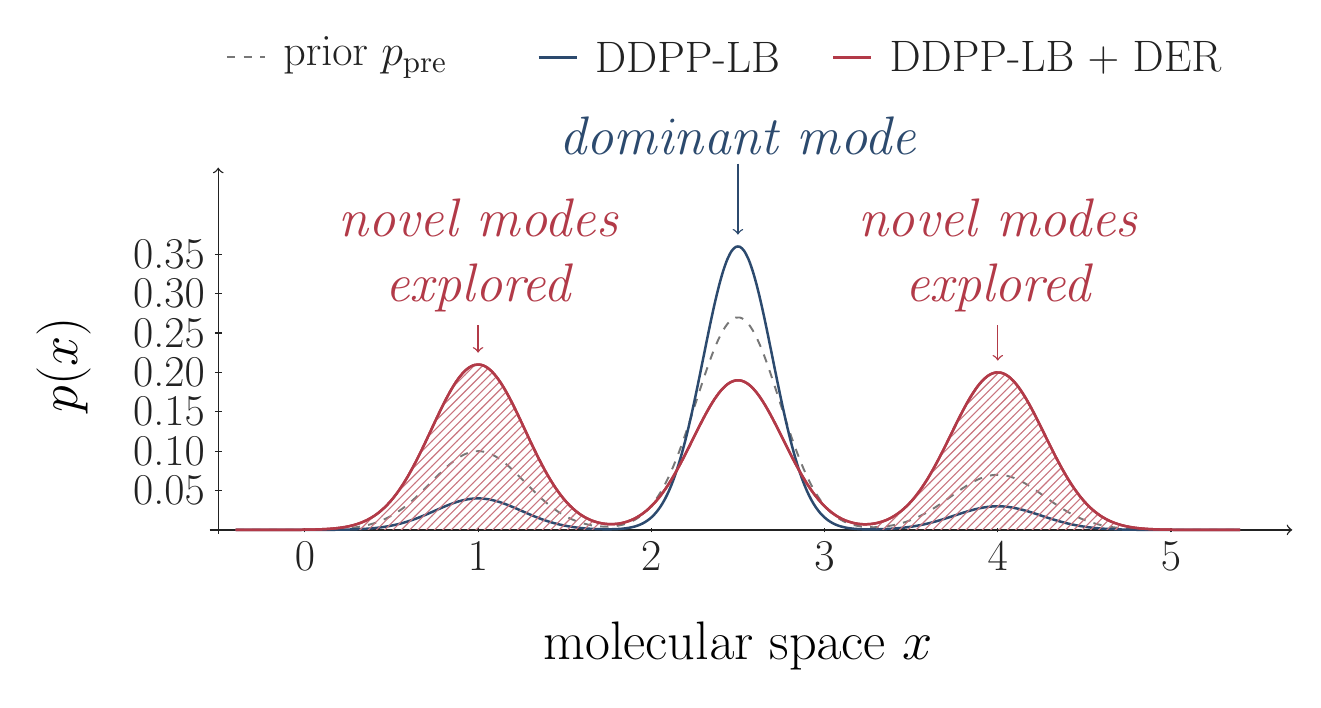
\begin{tikzpicture}[x=2.2cm, y=10cm]

  % Plot frame: x in [-0.5, 5.5], y in [0, 0.40]; three modes at x = 1, 2.5, 4

  \draw[->, line width=0.5pt, color=cInk] (-0.55, 0)    -- (5.7, 0);
  \draw[->, line width=0.5pt, color=cInk] (-0.50,-0.005) -- (-0.50, 0.46);
  \node[font=\small, anchor=north] at (2.5, -0.105) {molecular space $x$};
  \node[font=\small, rotate=90, anchor=south] at (-1.18, 0.21) {$p(x)$};

  \foreach \y/\lab in {0.05/0.05, 0.10/0.10, 0.15/0.15, 0.20/0.20, 0.25/0.25, 0.30/0.30, 0.35/0.35}{
    \draw[line width=0.4pt, color=cInk] (-0.52,\y) -- (-0.48,\y);
    \node[font=\scriptsize, color=cInk, anchor=east, xshift=-0.05cm] at (-0.50,\y) {\lab};
  }
  \foreach \x in {0,1,2,3,4,5}{
    \draw[line width=0.4pt, color=cInk] (\x,-0.003) -- (\x, 0.003);
    \node[font=\scriptsize, color=cInk, anchor=north] at (\x,-0.003) {\x};
  }

  % --- prior p_pre (gray dashed) ---
  \draw[dashed, line width=0.7pt, color=cMute, smooth, samples=240, domain=-0.4:5.4]
        plot (\x, {0.10 * exp(-0.5*((\x-1.0)/0.27)^2)
                 + 0.27 * exp(-0.5*((\x-2.5)/0.24)^2)
                 + 0.07 * exp(-0.5*((\x-4.0)/0.27)^2)});

  % --- DDPP-LB no debias (blue): dominant mode sharpens, minor modes shrink ---
  \draw[line width=0.9pt, color=cAccent, smooth, samples=240, domain=-0.4:5.4]
        plot (\x, {0.04 * exp(-0.5*((\x-1.0)/0.25)^2)
                 + 0.36 * exp(-0.5*((\x-2.5)/0.20)^2)
                 + 0.03 * exp(-0.5*((\x-4.0)/0.25)^2)});

  % --- DDPP-LB + neg-score (red): three modes more equal, minor modes lifted ---
  \draw[line width=0.9pt, color=cAccent2, smooth, samples=240, domain=-0.4:5.4]
        plot (\x, {0.21 * exp(-0.5*((\x-1.0)/0.27)^2)
                 + 0.19 * exp(-0.5*((\x-2.5)/0.26)^2)
                 + 0.20 * exp(-0.5*((\x-4.0)/0.27)^2)});

  % Hatched red wash on the LEFT and RIGHT minor modes (lift over prior)
  \begin{scope}
    \clip (0.3, 0) rectangle (1.7, 0.42);
    \fill[cAccent2Soft, pattern=north east lines, pattern color=cAccent2!70,
          smooth, samples=120, domain=0.3:1.7]
          plot (\x, {0.21 * exp(-0.5*((\x-1.0)/0.27)^2)})
          -- (1.7, 0) -- (0.3, 0) -- cycle;
  \end{scope}
  \begin{scope}
    \clip (3.3, 0) rectangle (4.7, 0.42);
    \fill[cAccent2Soft, pattern=north east lines, pattern color=cAccent2!70,
          smooth, samples=120, domain=3.3:4.7]
          plot (\x, {0.20 * exp(-0.5*((\x-4.0)/0.27)^2)})
          -- (4.7, 0) -- (3.3, 0) -- cycle;
  \end{scope}

  % Re-stroke red on top so hatching doesn't cover it
  \draw[line width=0.9pt, color=cAccent2, smooth, samples=240, domain=-0.4:5.4]
        plot (\x, {0.21 * exp(-0.5*((\x-1.0)/0.27)^2)
                 + 0.19 * exp(-0.5*((\x-2.5)/0.26)^2)
                 + 0.20 * exp(-0.5*((\x-4.0)/0.27)^2)});

  % Annotations
  \node[font=\small\itshape, color=cAccent2, anchor=south, align=center] at (1.0, 0.265)
        {novel modes\\explored};
  \draw[->, line width=0.5pt, color=cAccent2] (1.0, 0.260) -- (1.0, 0.225);

  \node[font=\small\itshape, color=cAccent2, anchor=south, align=center] at (4.0, 0.265)
        {novel modes\\explored};
  \draw[->, line width=0.5pt, color=cAccent2] (4.0, 0.260) -- (4.0, 0.215);

  \draw[->, line width=0.5pt, color=cAccent] (2.5, 0.465) -- (2.5, 0.375);
  \node[font=\small\itshape, color=cAccent, anchor=south] at (2.5, 0.465) {dominant mode};

  % Legend (top right)
  \begin{scope}[shift={(-0.45, 0.60)}]
    \draw[dashed, line width=0.7pt, color=cMute] (0.00, 0) -- (0.22, 0);
    \node[font=\scriptsize, color=cInk, anchor=west] at (0.27, 0) {prior $p_{\mathrm{pre}}$};
    \draw[line width=0.9pt, color=cAccent] (1.80, 0) -- (2.02, 0);
    \node[font=\scriptsize, color=cInk, anchor=west] at (2.07, 0) {DDPP-LB};
    \draw[line width=0.9pt, color=cAccent2] (3.50, 0) -- (3.72, 0);
    \node[font=\scriptsize, color=cInk, anchor=west] at (3.77, 0) {DDPP-LB $+$ DER};
  \end{scope}

\end{tikzpicture}
\end{document}
